\chapter{Introduction}

There is an organic rankine cycle (ORC) experiment setup located in the BURET (Bogazici University Renewable Energy Technologies) in Kilyos, Istanbul (See Figure \ref{exsetup}). The ORC setup's primary objective is to extract energy from low-temperature heat sources such as solar, waste, or biomass by using fluids with low boiling temperatures. The setup consists of two separate fluid cycles: the main working fluid cycle and the oil cycle. The oil cycle extracts energy from a heater and transfers the energy to the main working fluid. Meanwhile, hot and pressurized main working fluid spends its energy rotating a shaft that generates electricity.

\begin{figure}[H]
		\centering
		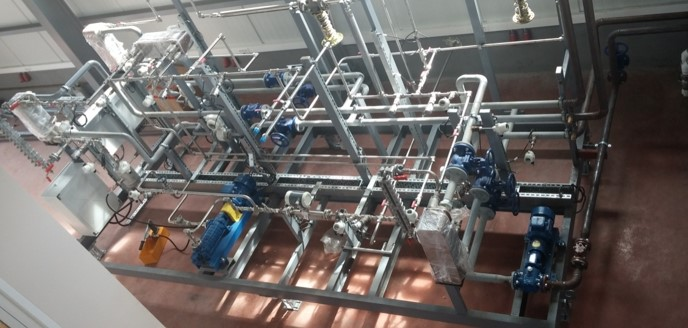
\includegraphics[width=0.6\textwidth]{images/exsetup.jpg}
		\caption[ORC Setup in BURET Lab]{ORC Setup in BURET Lab}
		\label{exsetup} 
\end{figure} 
	
The main working fluid cycle had already been investigated by Altun et al. Altun developed a dynamic simulation model that predicts the temperatures and pressures across the cycle, including the pressure and heat losses, by using Modelica and validated his model with the experiment results of the ORC setup. In this project, we focus on the other side of the ORC, the oil cycle, and we propose a way to improve the cycle.
	
The oil cycle (See Figure \ref{cycle}) consists of 4 main components: the heater, the pump, the evaporator, and the oil tank. Basically, the oil is heated at the heater, which has a resistor and an on-off temperature control unit. The hot oil is pumped toward the evaporator by a gear pump, and the oil transfers its energy to the cold main working fluid inside the evaporator, which is a plate-type heat exchanger. The heater can be controlled by setting a temperature. When the thermocouple at the exit of the heater determines a higher temperature than the set temperature, the heater is closed. When the temperature at the exit of the heater is determined to be less than the set temperature, the heater is turned on.
	
	\begin{figure}[H]
		\centering
		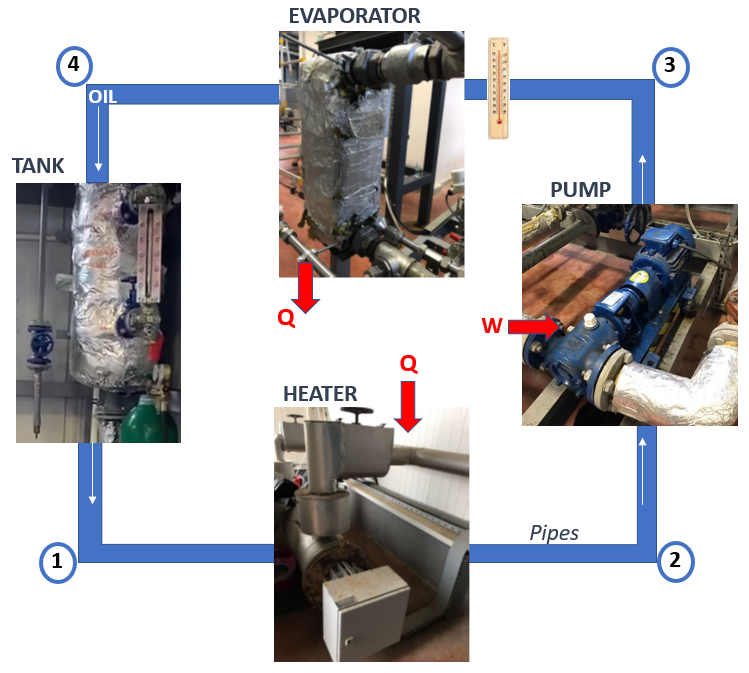
\includegraphics[width=0.56\textwidth]{images/cycle.png}
		\caption[The Oil Cycle]{The Oil Cycle}
		\label{cycle} 
	\end{figure} 
	
The problem that is aimed to be fixed in this project occurs because of the oil heater's on-off type temperature controller. The thermocouple used to determine the exit temperature at the exit has a hysteresis of $\pm 3^\circ C$. That is why the oil is either heated or left to be cooled much more than the desired set temperature. Additionally, the resistor inside the heater, which has a heating capacity of 100 kW, remains hot even after the heater is closed, resulting in an additional temperature rise after the set temperature is reached. Both of these reasons result in the oscillation of the oil temperature at the heater exit (See Figure \ref{osc}). The oscillation temperature of the oil causes the temperature of the main working fluid to oscillate.

\begin{figure}[H]
		\centering
		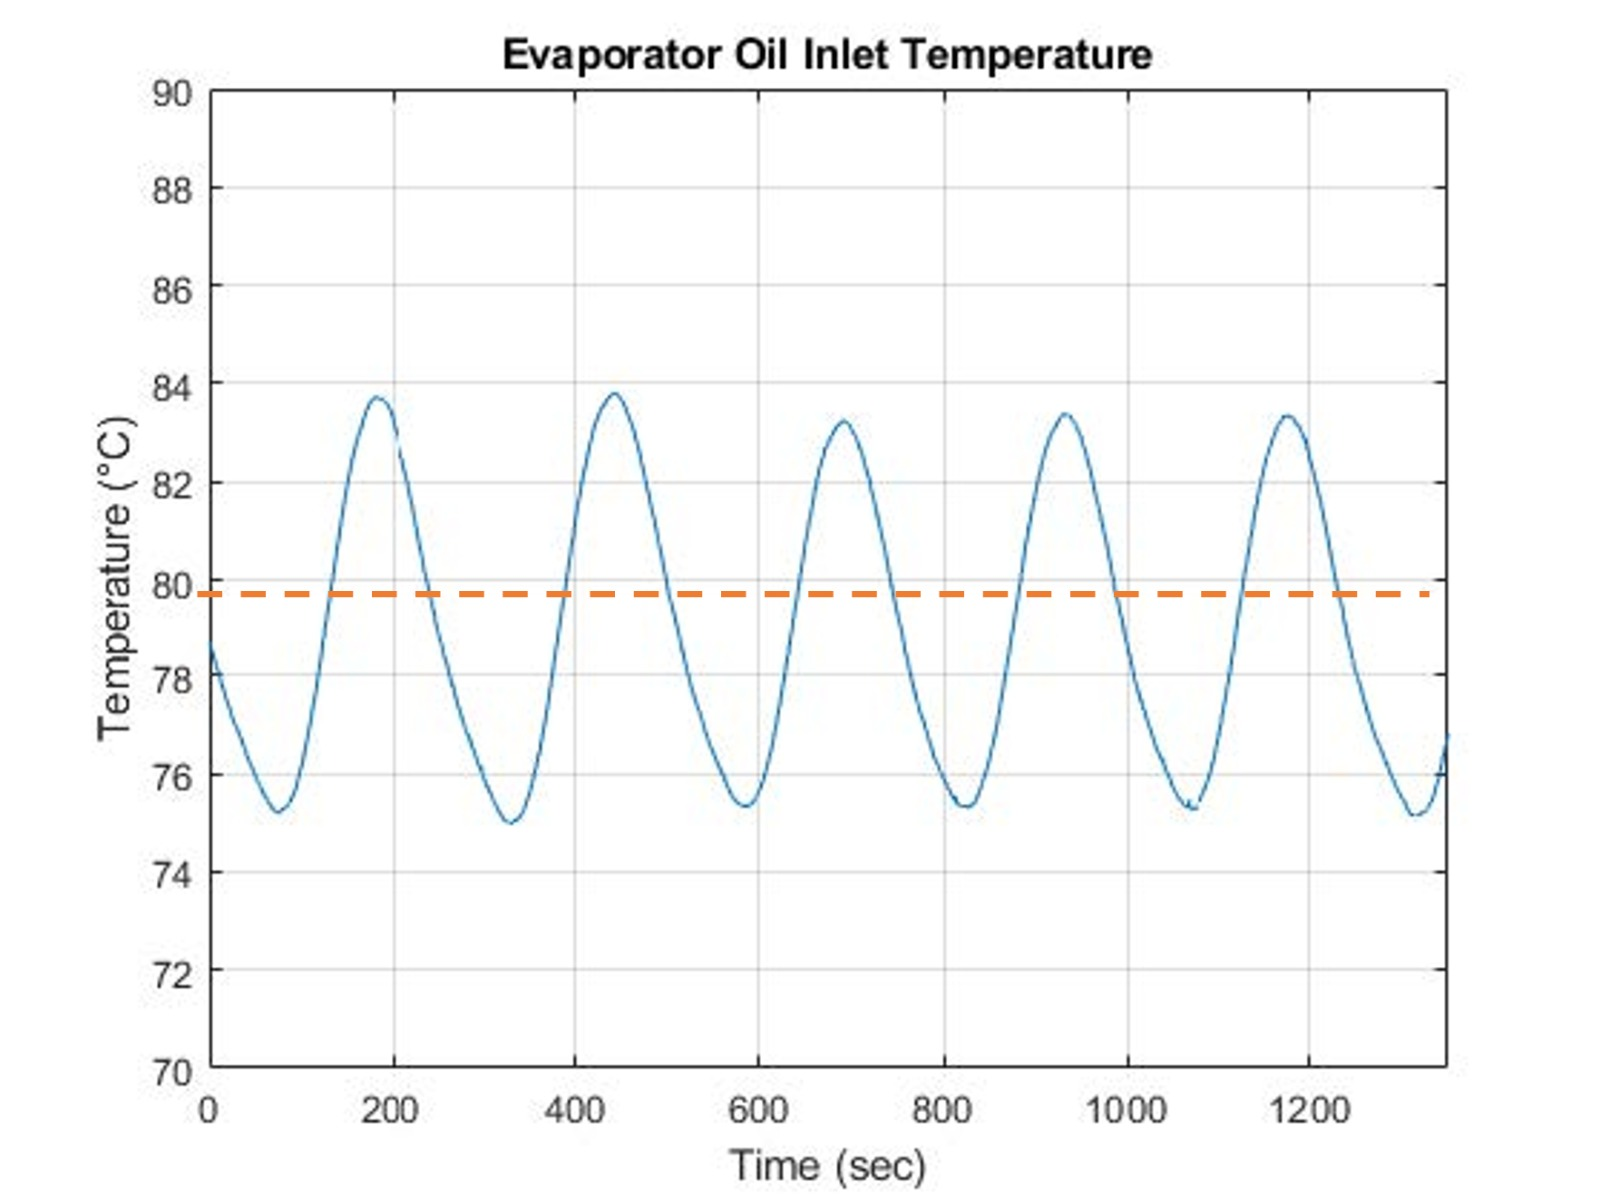
\includegraphics[width=0.6\textwidth]{images/oscillation.jpg}
		\caption[The oscillation of oil's temperature when set temperature is $80^\circ C$] {The Oscillation of Oil's temperature when set Temperature is $80^\circ C$}
		\label{osc} 
\end{figure} 

This project aims to develop a simulation model that predicts temperature across the oil cycle, propose a mechanical solution to decrease the oil oscillation, and modeling of the proposed solution. According to the literature, there is a couple of software that can be used to model a thermodynamic cycle, like ORC setups such as GtSuite, Modelica, and Matlab/Simulink.
	
An example study on the dynamic modeling of ORC and optimization of some components, such as turbines and heat exchangers, was conducted by Marchionni et al. \cite{marchi}. A 1D computer-aided modeling software called GTSuite was employed in his model. Rather than MW scale ORC systems, this research concentrates on kW scale systems. The goal of this study is to model ORC systems with power output ranging from 34.5 kW to 55.5 kW. To observe the cycle's transient reaction, various mass flow rates and intake temperatures of cooling water and hot oil are investigated.
	
Another software that can be employed to make a dynamic model for ORC is Modelica which is used by Wei et al. \cite{wei}. The cycle's heat source is a power plant's exhaust gas, and the air is used for cooling. They examined the accuracy, complexity, and simulation durations of moving boundary (MB) and finite volume (FV) methods. Results of the transient analysis are presented for both scenarios and contrasted with experimental data. It is discovered that the MB strategy is quicker and simpler than the FV approach as a result. The FV method, however, is more precise than the MB one. As a result, MB is more appropriate than the FV technique if the simulation time is the primary concern, whereas the FV approach would make more sense if it is not. Additional to Wei et al.'s study, Modelica/Dymola was used by Zhang et al. \cite{zhang}. to develop a dynamic model for kW scale ORC. Their steps were to model the components of ORC first and then compare the model's simulation results with the experiment results. As it turned out, the model's result was compatible with the results of the experiments. By validating the model, they also validated the thermal efficiency that they calculated by this model, which was 6.94\%. Other users of Modelica/Dynamo for ORC modeling were Quolin et al. \cite{quoilin}. They also compared the model results with the experiment results, and they discovered that the model was accurate. Ertugrul's research can be considered the predecessor of this project \cite{altun}. In his thesis, which is about dynamic modeling of the ORC setup (except the oil cycle section), he made a transient simulation of ORC and found out the temperature of the R134a across the ORC cycle by using Modelica/Dymola. He also considered simulating pressure losses across ORC and validated the results with the readings from the pressure sensor in ORC. Unlike his study, we neglected the pressure effects on the system since their effects are small, and it would be costly to implement pressure sensors in the oil cycle for validation.
	
Matlab/Simulink is another applicable software for the dynamic modeling of ORC. Carraro et al. \cite{carr}. made a study targeting to model and design of a small ORC setup with the help of Matlab. They investigated the ORC system's response to the oscillating temperature of the oil between 410 K and 435 K. When they compared their dynamic model's results with the experiment's results; they calculated the maximum relative error of 6.6\%.

A similar problem is solved by Akmal et al. \cite{inproceedings}. They used Matlab/Simulink to dynamically model an underfloor heating system that has an on-off type resistor. Their aim was to create a valid model that could optimize the heating of a room with underfloor heating. Similar to the heater in the oil cycle, the heater of the underfloor heating system overshoots or undershoots the set temperature because of the delayed response of the resistor.
	
As can be seen, there are many ways to create a dynamic model of a part of the ORC setup. Modelica/Dymola, GT-Suite, and Matlab/Simulink are generally used for this purpose, and they give compatible results with the results of the experiment. In this project, Matlab/Simulink is chosen to model the oil cycle. This is mainly because of time scarcity since Matlab/Simulink is a more familiar software for us, and it would take time to learn new software. Additionally, Simulink's easy-to-use and practical interface is beneficial for us.